\section{Solver Configuration}

A solver(s) is required to solve the VI model, and a few considerations need to be taken into account when choosing one.
For choosing and motivating a solver configuration, the \textit{COMSOL Multiphysics Reference Manual v5.3a}\cite{comsol_comsol_nodate} is here continuously used as a source.\par

For simplicity we will now first consider a stationary or steady-state problem.
Since our model is a multiphysics problem, i.e. many of the physical parameters depend on each other, we first need consider how to couple them.
They can be coupled by either using a \textit{segregated} or \textit{fully coupled} approach.\par

\paragraph{Segregated vs. fully coupled physics}

In a segregated solver, each governing equation is solved separately in a specific order.
For instance, in our VI example we can solve Darcy's Law first, get some solution for airflow in soil, and then use that velocity field in the transport equation, solve that, and then solve the indoor concentration equation, i.e. we solve one system equation per step.
These steps are simply iterated until convergence occurs in all of the separated steps.
In the case of VI calculations, the use of the segregated approach is fully justified because the concentrations of contaminant vapors are normally so low that they have no impact on the solution of soil airflow using Darcy's Law.
The fully coupled approach assembles a single large system of equations.
Both of these approaches should reach the same solution, but the fully coupled approach will do so faster, but at the expense of using more memory.\par

\paragraph{Direct vs. iterative solver}

Within each of these coupling approaches, we need to specify a solver to solve the system of equations.
Here we are again faced with a choice, and we could either use a \textit{direct} or \textit{iterative} solver.
Direct solvers, as the name implies, arrive at a solution directly and are based on LU-decomposition.
Iterative solvers on the other hand, iteratively approach the solution, and are based on conjugate gradient method.
The advantage of direct solvers is that they are faster, but use more memory, while iterative solvers are slower but use less memory.
In terms of choosing a solver algorithm, there are many options, but MUMPS and GMRES will be used as the respective algorithm for direct and iterative solvers.\par

\paragraph{Time-dependent solvers}

To solve a transient or time-dependent problem (which will be done in subsequent chapters) a solver to step forward in time is required.
Too large a time step will cause stability issues and ultimately convergence will be impossible, but obviously some discrete time step is required for a solution to be achievable.
A time-dependent solver picks an appropriate time-step and there are some popular approaches, such as using some high-order Runge-Kutta (RK) or backwards differentiation formula (BDF).
Regardless of the type of solver, for each time step the system of equations will be solved using one of the aforementioned solvers.
The difference between RK and BDF is that RK explicitly discretizes time while BDF does so implicitly.
In this work we will only use BDF as it is more stable than RK.\par

\paragraph{Choosing solvers}

The choice of solver will not affect (or should not at least) the solution to the problem.
However, it can have a large impact on computational time and resources, and these considerations dictate solver choice (this is also partially dependent on the mesh used, as this will affect memory usage too).
In this example, and throughout the models used in this work, we will favor speed over memory and therefore fully couple all our equations and use direct solvers.\par

\subsection{Adaptive Mesh Refinement}

The accuracy of the solution obtained by FEM is dependent on the quality of the mesh, something that was discussed in section \ref{sec:meshing}.
While the mesh designer can do much to create a mesh that performs well for the particular problem posed, refinement of the mesh is often needed and should be performed for every new model.\par

There are two types of mesh refinements in FEM.
The first type reduces the size of the elements and thereby the accuracy of the solution, this is called \textit{h-type} refinement ($h$ is often used to denote the mesh size).
The second increases the order of the polynomial of the basis function, called \textit{p-type} refinement which will likewise increases the solution accuracy.\par

h-type refinement is generally more attractive because it is simpler and the computational cost of p-type refinement increase faster than h-type.
However, p-types are useful if the user imports an already existing mesh, and is unable to change it, rendering h-type refinement impossible.
These two method can be combined to perform a \textit{hp-type} refinement.\par

Refinement is usually done by an algorithm, which is possible because FEM has the built-in ability to estimate the local error of the solution anywhere in the domain.
The downside with using an algorithm is that the user has little control over how the mesh is refined.
The user can also manually refine the mesh by solving the model and plot how some relevant metric converges as the mesh is refined.
This can be a very time consuming, and therefore algorithms are usually preferable; a hybrid solution is to manually alter the mesh after the algorithmic mesh refinement.\par

Refinement can either be done locally or globally.
Global refinement involves defining some singular metric that will be used to evaluate the quality of the mesh, e.g. one might use the total stress in a metal bar as a metric here.
In local refinement, one still has to define some metric for evaluating the quality of the refinement, but evaluation only occurs on a subset of the domain, e.g. the stress on just one boundary of the same metal bar.
In both approaches the elements that have the largest estimated local relative error are refined, but the exact details of the refinement can differ between specific refinement algorithms.
The local relative error is defined as the difference of the approximated solution $u_h$ from one mesh to another.
\begin{equation}\label{eq:rel_error}
  e = u_{h1} - u_h
\end{equation}
$e$ is the estimated local relative error (for every node);
$u_{h1}$ and $u_h$ are the approximated solutions on the refined and original meshes respectively.
The optimal type of refinement varies by problem, but a global refinement will generally be more computationally expensive.\par

\begin{figure}[htb!]
  \centering
  \begin{subfigure}[b]{\textwidth}
    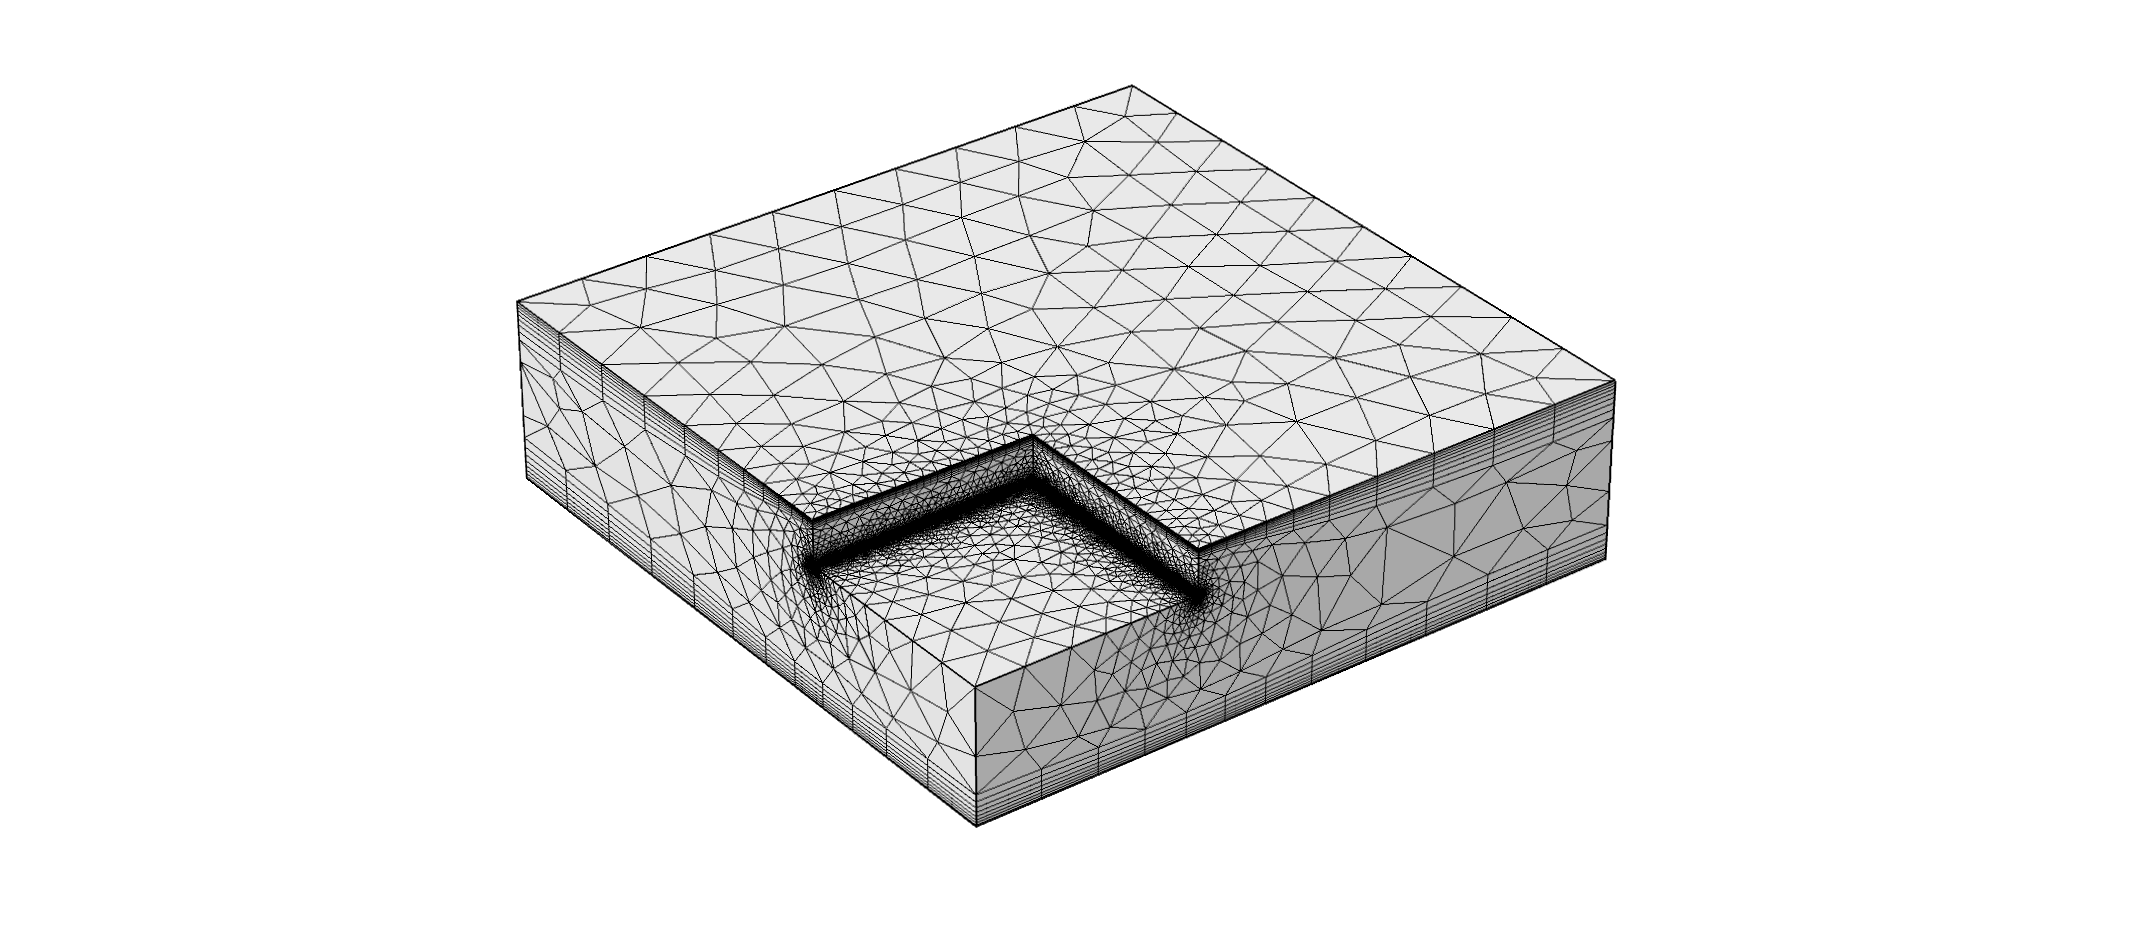
\includegraphics[width=\textwidth]{meshed_model.png}
    \caption{Original mesh. 362,657 elements.}
    \label{fig:mesh_before_refinement}
  \end{subfigure}
  \begin{subfigure}[b]{\textwidth}
    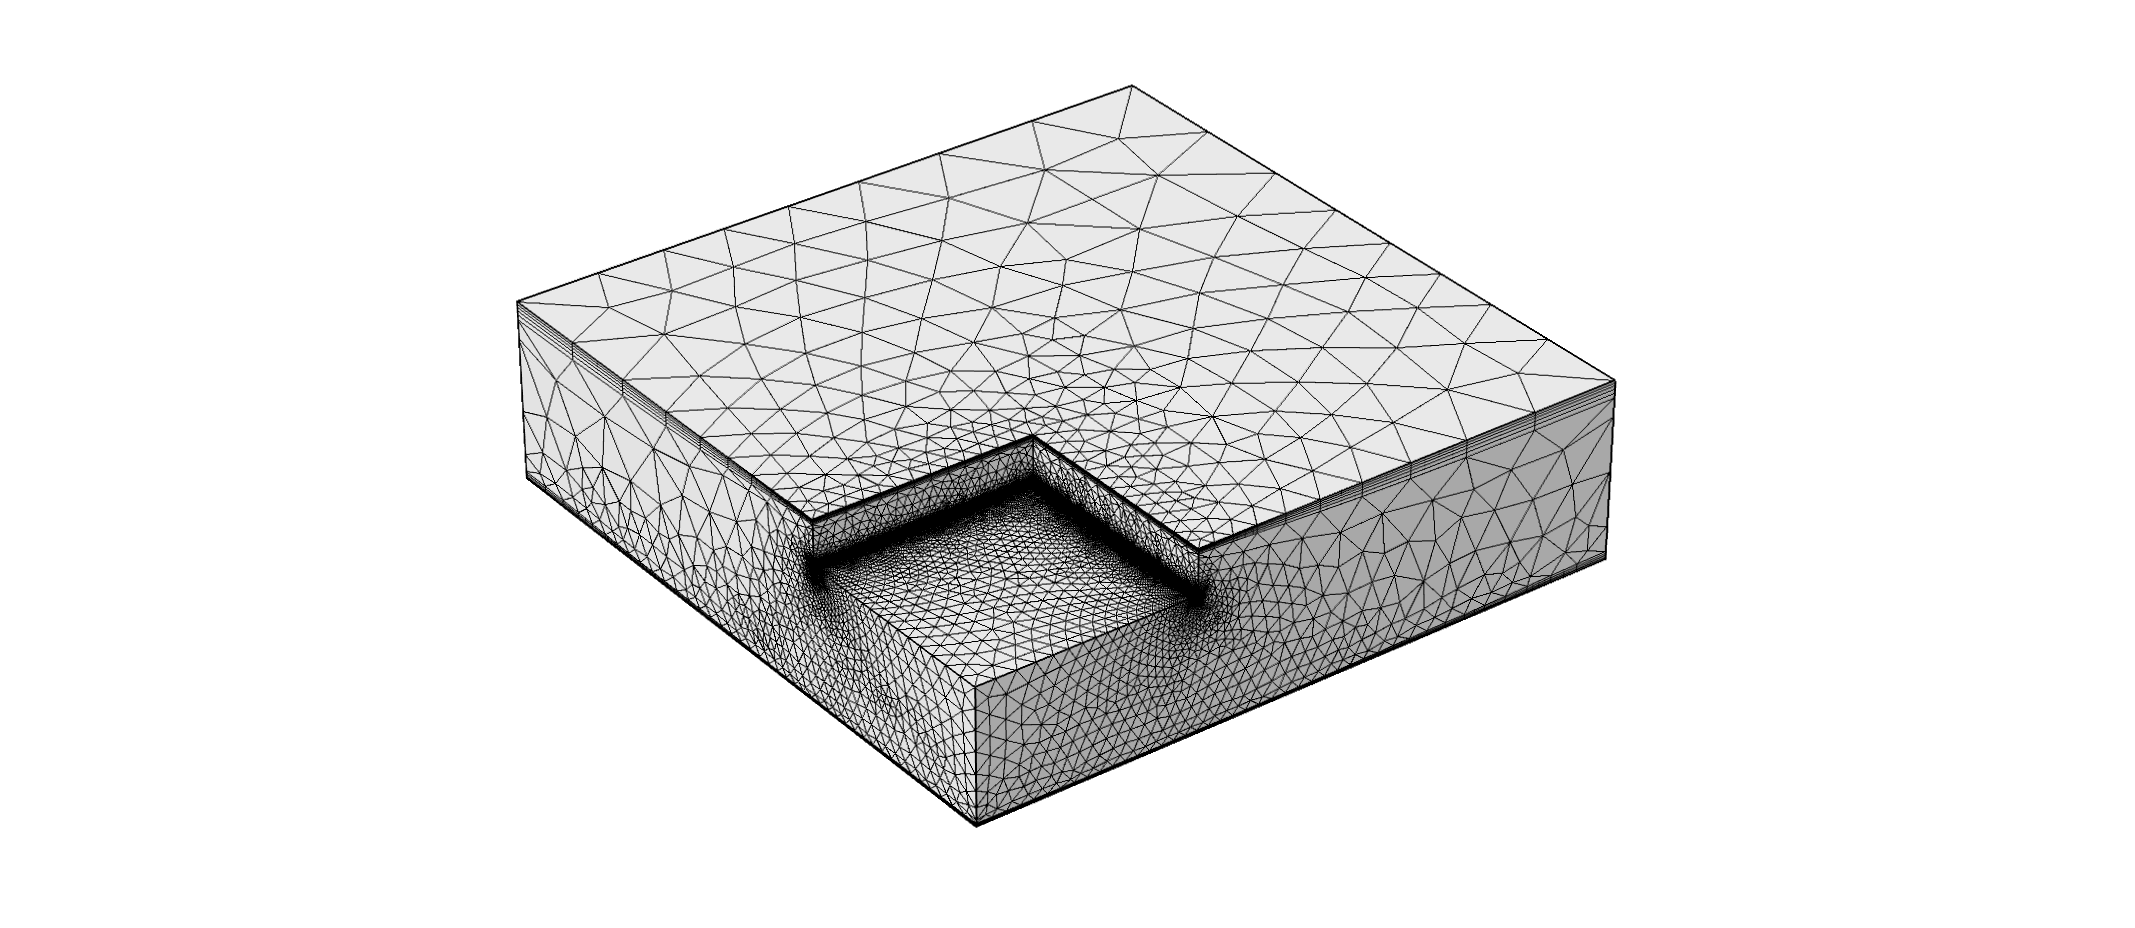
\includegraphics[width=\textwidth]{mesh_refined.png}
    \caption{Refined mesh after global refinement w.r.t. the indoor contaminant concentration. 1,065,743 elements.}
    \label{fig:mesh_after_refinement}
  \end{subfigure}
    \caption[Original and adaptatively refined mesh.]{Original and adaptatively refined mesh.}
    \label{fig:mesh_refinement_mesh}
\end{figure}

In this work we will use a global h-type refinement and use the indoor contaminant concentration $c_{in}$ as our refinement metric.
COMSOLs refinement algorithm has the nice ability to reinitialize the mesh, and can thereby coarsen elements, i.e. increase $h$ where the local error is very small.
This is handy as a fine mesh is not needed far away from the foundation crack - saving computational resources.
In this example we will tell the algorithm to refine the mesh three times, and stop if the total number of elements exceed 1 million, with a maximum coarsening factor of 3, and element growth rate of 1.3, i.e. the number of elements increase by roughly 70\% each iteration.\par

The result of this refinement can be seen in Figure \ref{fig:mesh_refinement_mesh} where the original and refined mesh are juxtaposed.
Notice how the mesh is now denser near the foundation, the boundary layers tighter (in particular near the groundwater boundary), and how the elements are larger in the periphery.
The original and refined meshes has 362,657 and 1,065,743 elements respectively.\par
Figure \ref{fig:mesh_refinement} shows how the value of $c_\mathrm{in}$ converges for each mesh refinement iteration.
What is plotted is the change in calculated indoor contaminant concentration with iteration.
Initially, very large changes are seen in the predicted values with the first iterations.
By the \nth{4} iteration, the improvements in estimates are getting very small.\par

\begin{figure}[htb!]
  \centering
  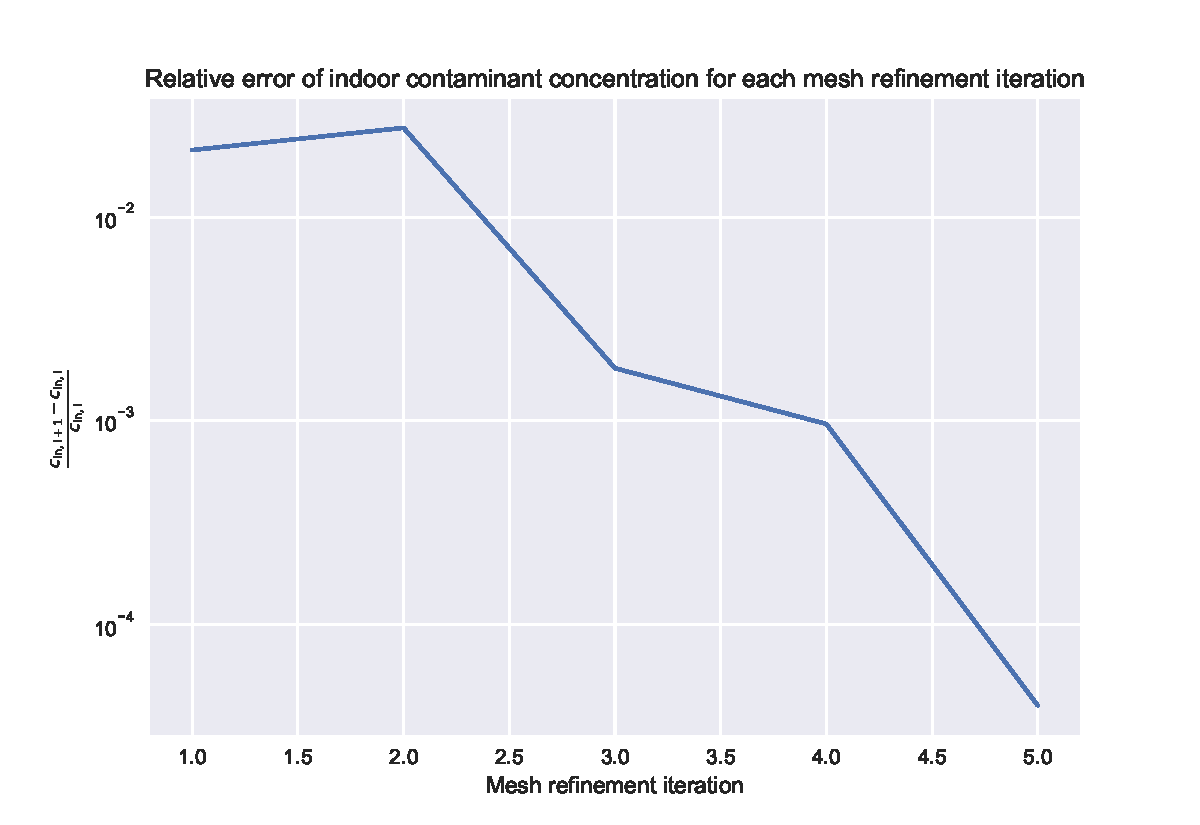
\includegraphics[width=0.75\textwidth]{mesh_refinement_error.pdf}
  \caption{Convergence of indoor air contaminant concentration as the mesh is refined.}
  \label{fig:mesh_refinement}
\end{figure}
